% !TEX root = main.tex
% 82 124 170 231
\subsection{Numerical Simulations}
In this section, we consider several situations that vehicles in a platoon on an air highway may commonly encounter, and show via simulations the behaviors that emerge from the controllers we defined in Sections \ref{sec:platooning}-\ref{sec:reach_ctrl} and \ref{sec:platooning}-\ref{sec:other_ctrl}.

\subsubsection{Forming a Platoon}
We first consider the scenario in which Free vehicles merge onto an initially unoccupied highway. In order to do this, each vehicle first checks safety with respect to all other vehicles, and uses the safety controller if necessary, according to Section \ref{sec:platooning}-\ref{sec:reach_ctrl}-\ref{sec:collision_ctrl}. Otherwise, the vehicle uses the liveness controller for getting to an absolute target set described in Section \ref{sec:platooning}-\ref{sec:reach_ctrl}-\ref{sec:abs_target_ctrl} in order to merge onto the highway, create a platoon, and become a Leader vehicle if there are no platoons on the highway. If there is already a platoon on the highway, then the vehicle would use the liveness controller for getting to a target set relative to the platoon leader as described in Section \ref{sec:platooning}-\ref{sec:reach_ctrl}-\ref{sec:rel_target_ctrl} to join the platoon and become a Follower.

For the simulation example, shown in Figure \ref{fig:fp}, the highway is specified by a line segment beginning at the origin. The five vehicles, $\veh{1}, \veh{2}, \ldots, \veh{5}$ are colored orange, purple, light blue, dark blue, and yellow, respectively.

The first two plots in Figure \ref{fig:fp} illustrate the use of liveness and safety reachable sets for the first two vehicles. Since the liveness reachable sets are in 4D and the safety reachable sets are in 6D, we compute and plot their 2D slices based on the vehicles' velocities and relative velocities.  All vehicles begin as Free vehicles, so they each need to take into account five different reachable sets: four safety reachable sets and one liveness reachable set. For clarity, we only show the liveness reachable set and the four safety reachable sets for one of the vehicles. 

For $\veh{1}$ (orange), an arbitrary point of entry on the highway is chosen as the target absolute position, and the velocity corresponding to a speed of $10$ m/s in the direction of the highway is chosen as the target absolute velocity. This forms the target state $\bar{x}_H=(\bar{p}_x, \bar{v}_x, \bar{p}_y, \bar{v}_y)$, from which we define the target set $\mathcal{L}_H$ as in Section \ref{sec:platooning}-\ref{sec:reach_ctrl}-\ref{sec:abs_target_ctrl}.

At $t=4.2$, $\veh{1}$ (orange) is inside the liveness reachable set for getting to an absolute state, shown as the dotted orange boundary. Therefore, it is ``locked-in" to the target state $\bar{x}_H$, and follows the optimal control in \eqref{eq:HJB_ctrl_syn} to $\bar{x}_H$. During the entire time, $\veh{1}$ checks whether it may collide with any of the other vehicles within a time horizon of $\td$. To do this, it simply checks whether its state relative to each of the other vehicles is within the corresponding safety reachable set. As an example, the safety reachable set boundary with respect to $\veh{2}$ (purple) is shown as the orange dashed boundary around $\veh{2}$ (purple); $\veh{1}$ (orange) is safe with respect to $\veh{2}$ (purple) since $\veh{1}$ (orange) is outside of the boundary. In fact, $\veh{1}$ is safe with respect to all vehicles.

After completing merging onto the empty highway, $\veh{1}$ (orange) creates a platoon and becomes its leader, while subsequent vehicles begin to form a platoon behind the leader in the order of ascending distance to $\veh{1}$ (orange) according to the process described in Section \ref{sec:platooning}-\ref{sec:reach_ctrl}-\ref{sec:rel_target_ctrl}. Here, we choose the target relative position $(\bar{p}_{x,r}, \bar{p}_{y,r})$ to be a distance $\sepdist$ behind the last reserved slot in the platoon, and the target relative velocity $(\bar{v}_{x,r}, \bar{v}_{y,r}) = (0,0)$ with respect to the leader in order to maintain the platoon formation. This gives us the target set $\mathcal{L}_P$ that we need.

At $t=8.0$, $Q_2$ (purple) is in the process of joining the platoon behind $\veh{1}$ (orange) by moving towards the target $\bar{x}_P$ relative to the position of $\veh{1}$ (orange). Note that $\bar{x}_P$ moves with $\veh{1}$ (orange) as $\bar{x}_P$ is defined in terms of the relative states of the two vehicles. Since $\veh{2}$ is inside the liveness reachable set boundary for joining the platoon (purple dotted boundary), it is ``locked-in" to the target relative state $\bar{x}_P$, and begins following the optimal control in \eqref{eq:HJI_ctrl_syn} towards the target as long as it stays out of all safety reachable sets. For example, at $t=5.9$, $\veh{2}$ (purple) is outside of the safety reachable set with respect to $\veh{1}$ (orange), shown as the purple dashed boundary around $\veh{1}$ (orange). Again, from the other safety reachable set boundaries, we can see that $\veh{2}$ is in fact safe with respect to all vehicles.

In the bottom plots of Figure \ref{fig:fp}, $\veh{1}$ (orange) and $\veh{2}$ (purple) have already become the platoon leader and follower, respectively. The rest of the vehicles follow the same process to join the platoon. All 5 vehicles eventually form a single platoon and travel along the highway together. As with the first two vehicles, the liveness controllers allow the remaining vehicles to optimally and smoothly join the platoon, while the safety controllers prevent collisions from occurring.

% 40 60 110 210
\begin{figure} 
    \centering
    \begin{subfigure}[t]{0.45\textwidth} \label{subfig:fp_43}
        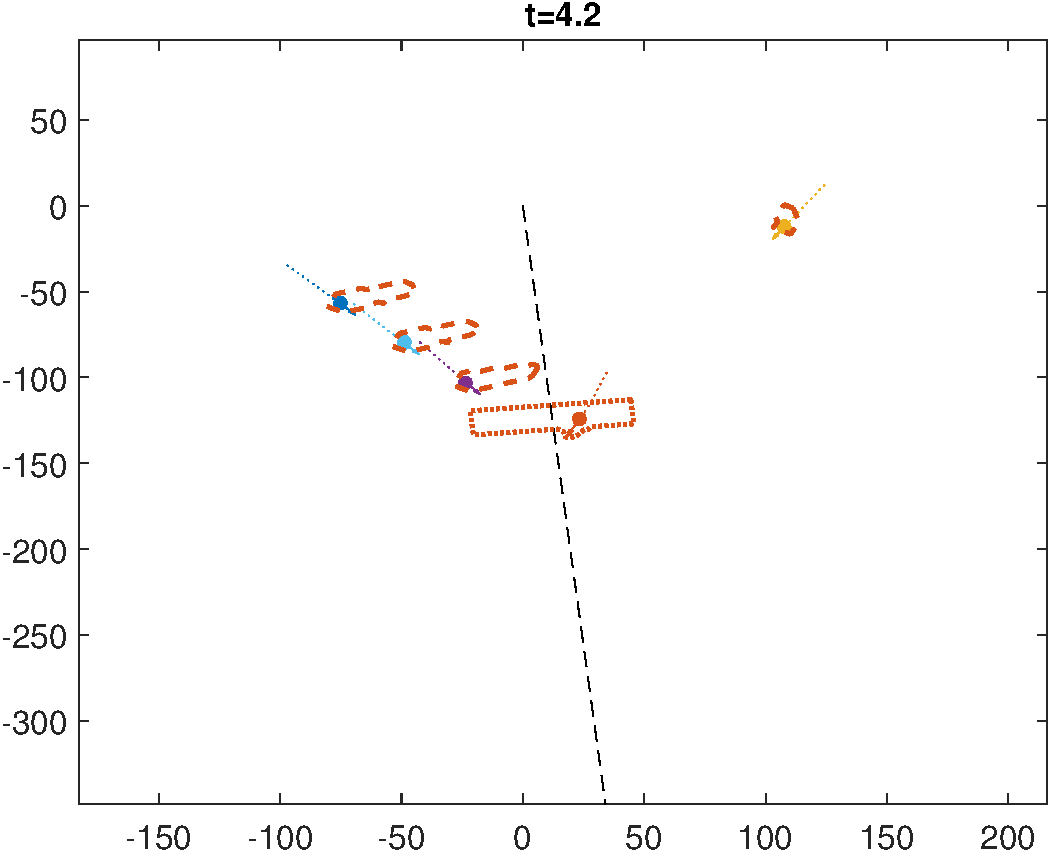
\includegraphics[width=\textwidth]{fig/fp_43}
        \caption{The red vehicle follows the reachability-based liveness controller for getting to an absolute target state to merge onto the highway, while avoiding collisions using the reachability-based safety controller. The liveness reachable set and one safety reachable set are shown as the dotted and dashed boundaries, respectively.}
    \end{subfigure}
    \begin{subfigure}[t]{0.45\textwidth} \label{subfig:fp_81}
        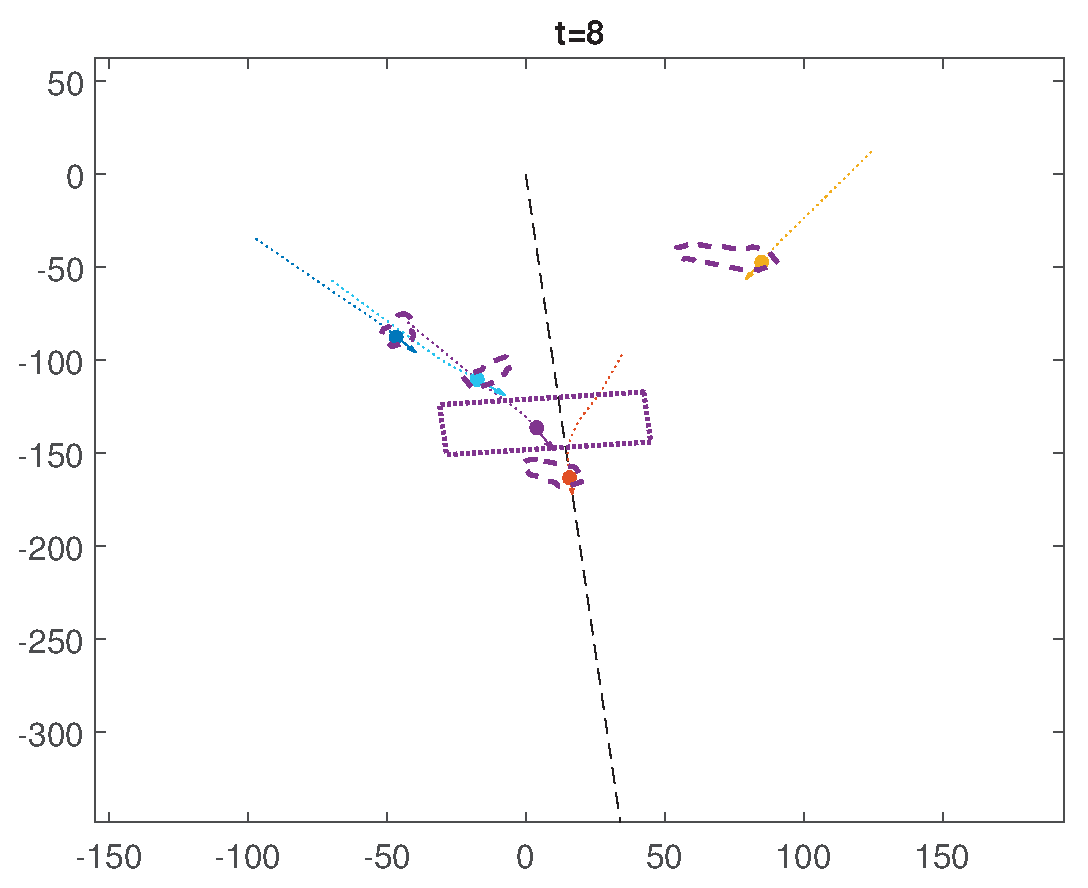
\includegraphics[width=\textwidth]{fig/fp_81}
        \caption{After the red vehicle successfully merges onto the highway and becomes the platoon leader, the purple vehicle uses the reachability-based liveness controller for getting to a relative target state to join the platoon, while avoiding collisions using the reachability-based safety controller. The liveness and safety reachable sets are shown as the dotted and dashed boundaries, respectively.}
    \end{subfigure}

    \begin{subfigure}[t]{0.45\textwidth} \label{subfig:fp_110}
        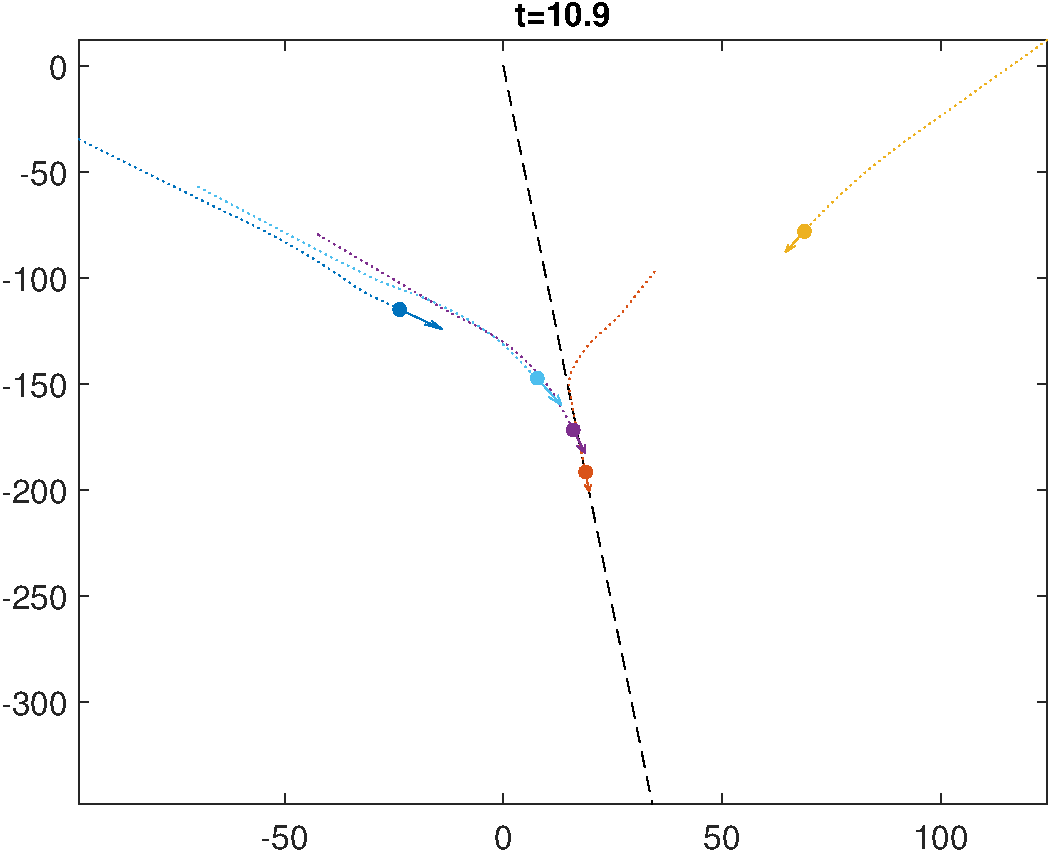
\includegraphics[width=\textwidth]{fig/fp_110}
        \caption{After the first two vehicles successfully form a two-vehicle platoon, the rest of the vehicles follow the same process to join the platoon.}
    \end{subfigure}
    \begin{subfigure}[t]{0.45\textwidth} \label{subfig:fp_210}
        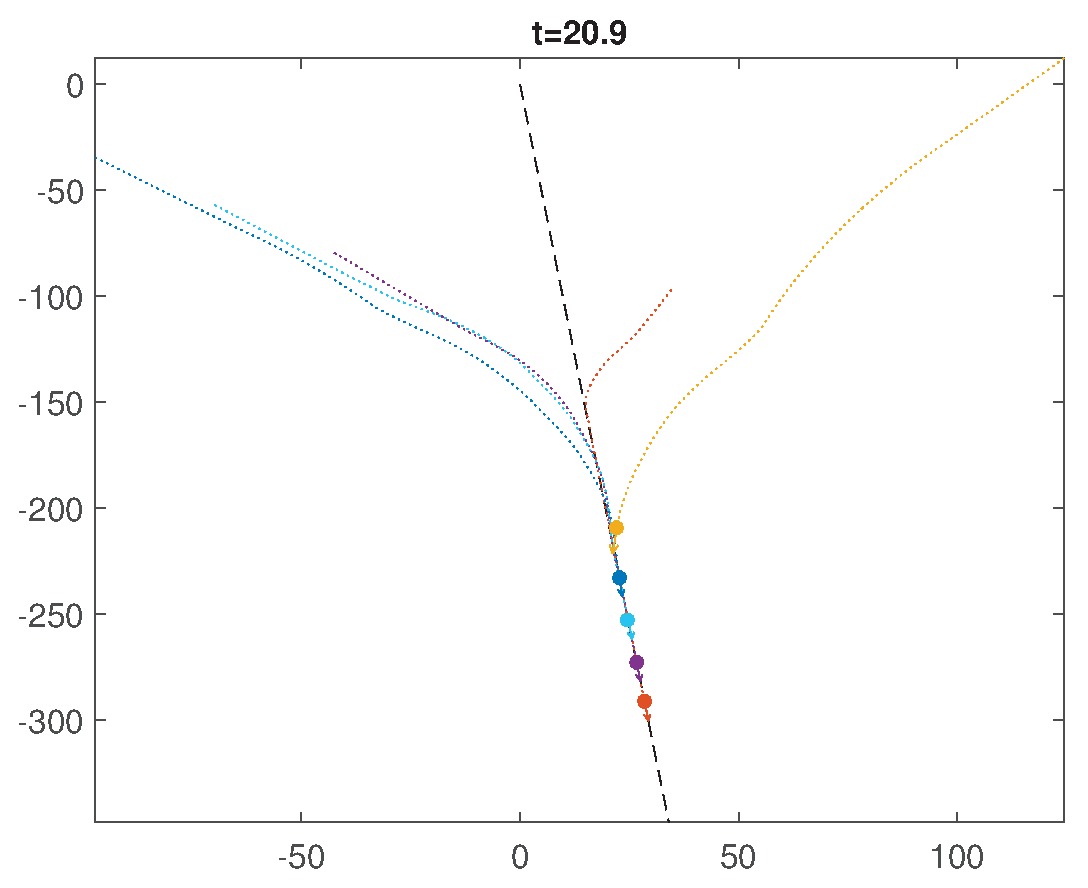
\includegraphics[width=\textwidth]{fig/fp_210}
        \caption{All five vehicles have successfully joined the platoon and now travel on the highway together.}
    \end{subfigure}   
    \caption{A simulation showing how five vehicles initially in the Free mode can form a platoon. \label{fig:fp}}
\end{figure}

\subsubsection{Intruder Vehicle}
We now consider the scenario in which a platoon of vehicles encounters an intruder vehicle. To avoid collision, each vehicle checks for safety with respect to the intruder and any vehicles in front and behind of it in the platoon. If necessary, the vehicle uses the reachability-based safety controller to avoid collision, otherwise it uses the appropriate controller to travel on the highway if it is a leader, or follow the leader if it is a follower. After danger has passed, the vehicles in the platoon resume normal operation.

Figure \ref{fig:in} shows the simulation result. At $t=9.9$, a platoon of four vehicles, $\veh{i},i=1,\ldots,4$ (with $P_i = i$), travels along the highway shown. An intruder vehicle $\veh{5}$ (yellow) heads left, disregarding the presence of the platoon. At $t=11.9$, the platoon leader $\veh{1}$ (red) detects that it has gone near the boundary of the safety reachable set (not shown) with respect to the intruder $\veh{5}$ (yellow). In response, $\veh{1}$ (red) starts using the safety controller to optimally avoid the intruder according to \eqref{eq:HJI_ctrl_syn}; in doing so, it steers slightly off the highway. 

Note that although in this particular simulation, the intruder travels in a straight line, a straight line motion of the intruder was \textit{not} assumed. Rather, the safety reachable sets are computed assuming the worst case control of the intruder, according to \eqref{eq:HJI_ctrl_syn}.

As the intruder $\veh{5}$ (yellow) continues to disregard other vehicles, the followers of the platoon also get near the respective boundaries of the safety reachable set with respect to the intruder. This occurs at $t=13.9$, where the platoon ``makes room'' for the intruder to pass by to avoid collisions; all vehicles deviate from their intended path, which is to follow the platoon leader or the highway.

After the intruder has passed, eventually all vehicles become far away from any safety reachable sets. When this occurs, the leader resumes following the highway, and the followers resume following the leader. At $t=19.9$, the platoon successfully gets back onto the highway.

% 100 120 140 200
\begin{figure}
    \centering
    \begin{subfigure}[t]{0.45\textwidth} \label{subfig:in_100}
        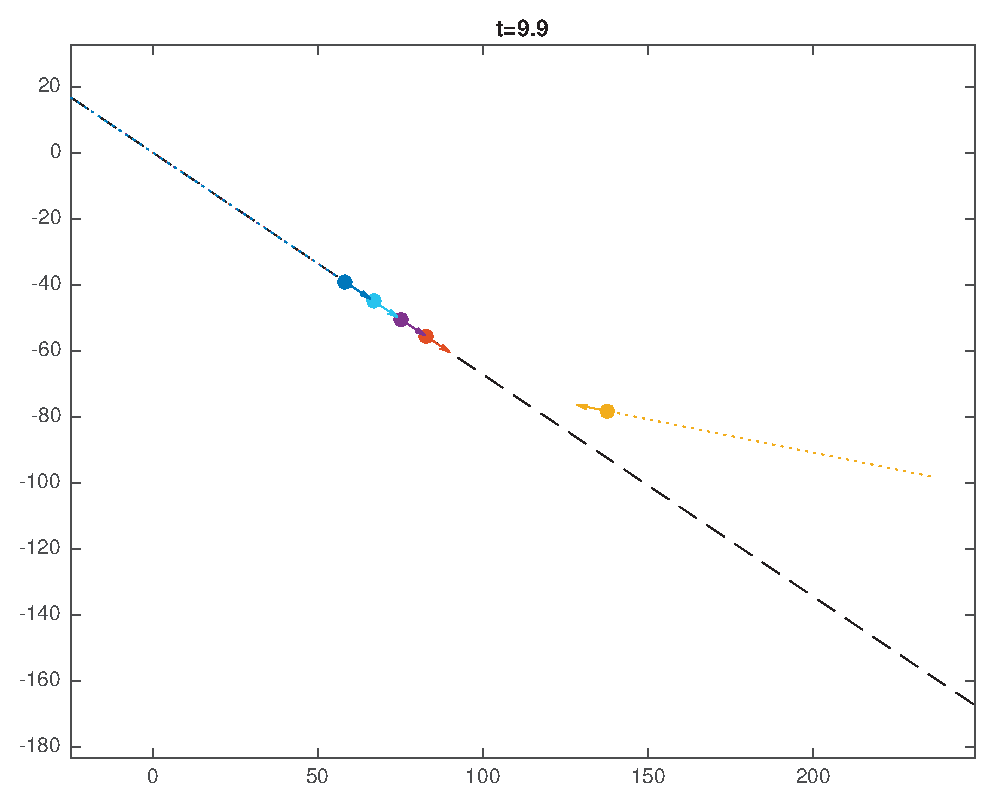
\includegraphics[width=\textwidth]{fig/in_100}
        \caption{Four vehicles in a platoon are traveling along the highway. The yellow intruder disregards other vehicles.}
    \end{subfigure}
    \begin{subfigure}[t]{0.45\textwidth} \label{subfig:in_120}
        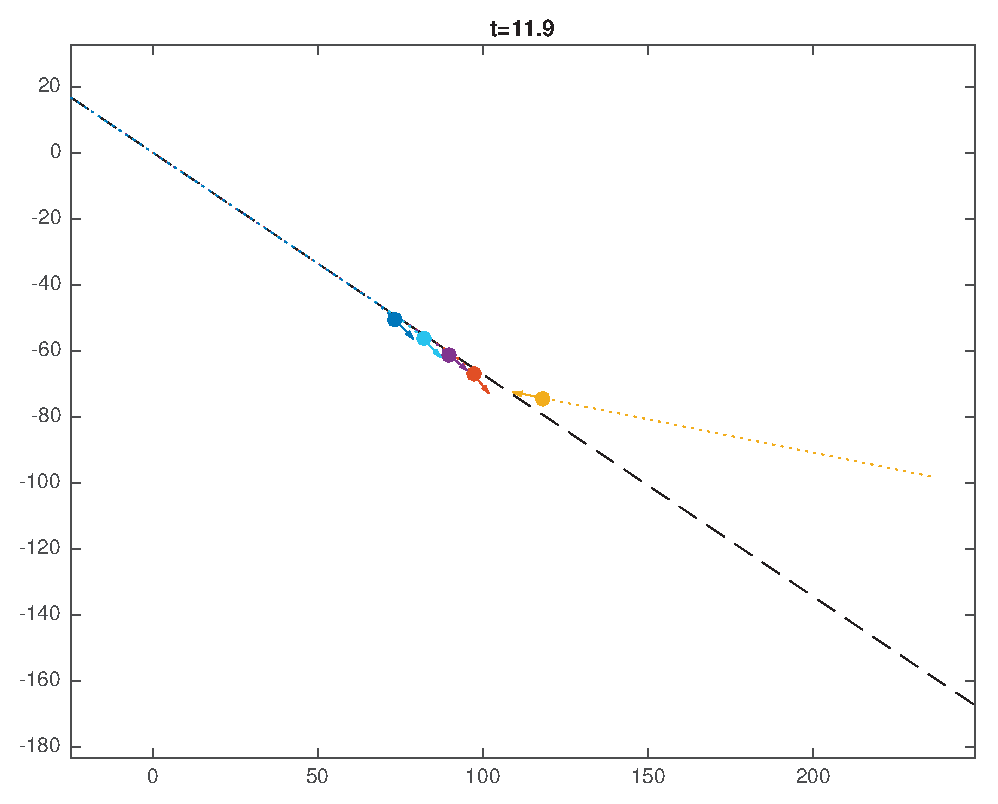
\includegraphics[width=\textwidth]{fig/in_120}
        \caption{Platoon members begin avoidance maneuvers as they get near the safety reachable set boundaries with respect to the intruder.}
    \end{subfigure}

    \begin{subfigure}[t]{0.45\textwidth} \label{subfig:in_140}
        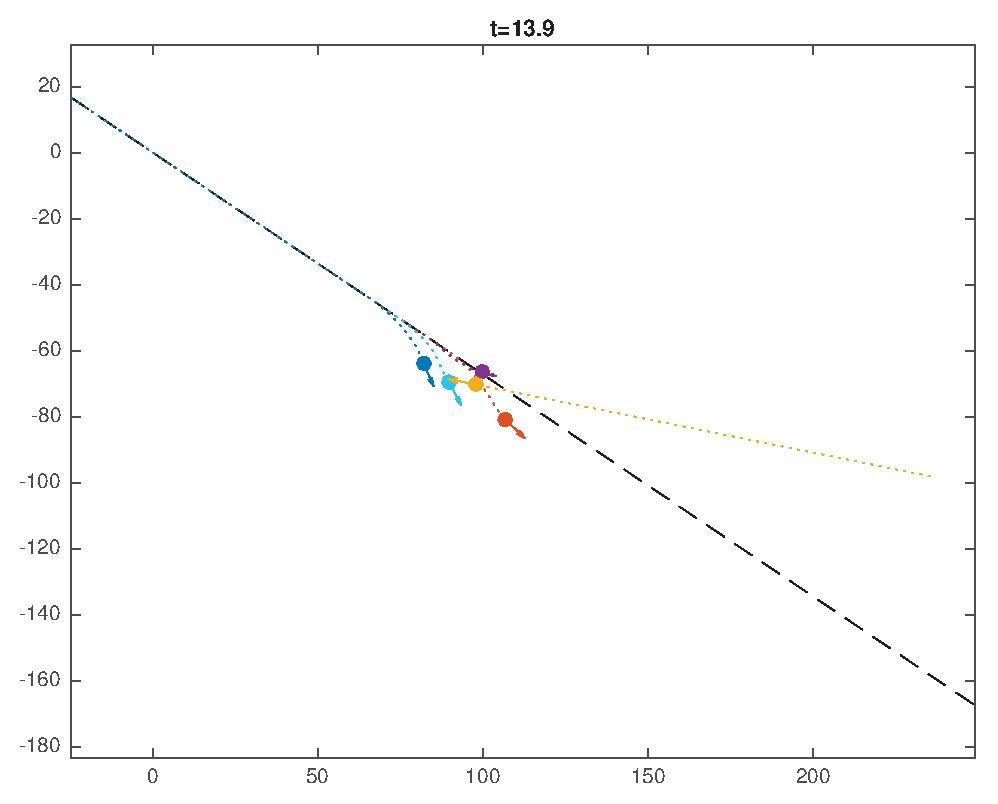
\includegraphics[width=\textwidth]{fig/in_140}
        \caption{As the intruder (yellow) crosses the highway, the safety controller causes platoon members spread out to ``make room'' for the intruder to pass.}
    \end{subfigure}
    \begin{subfigure}[t]{0.45\textwidth} \label{subfig:in_200}
        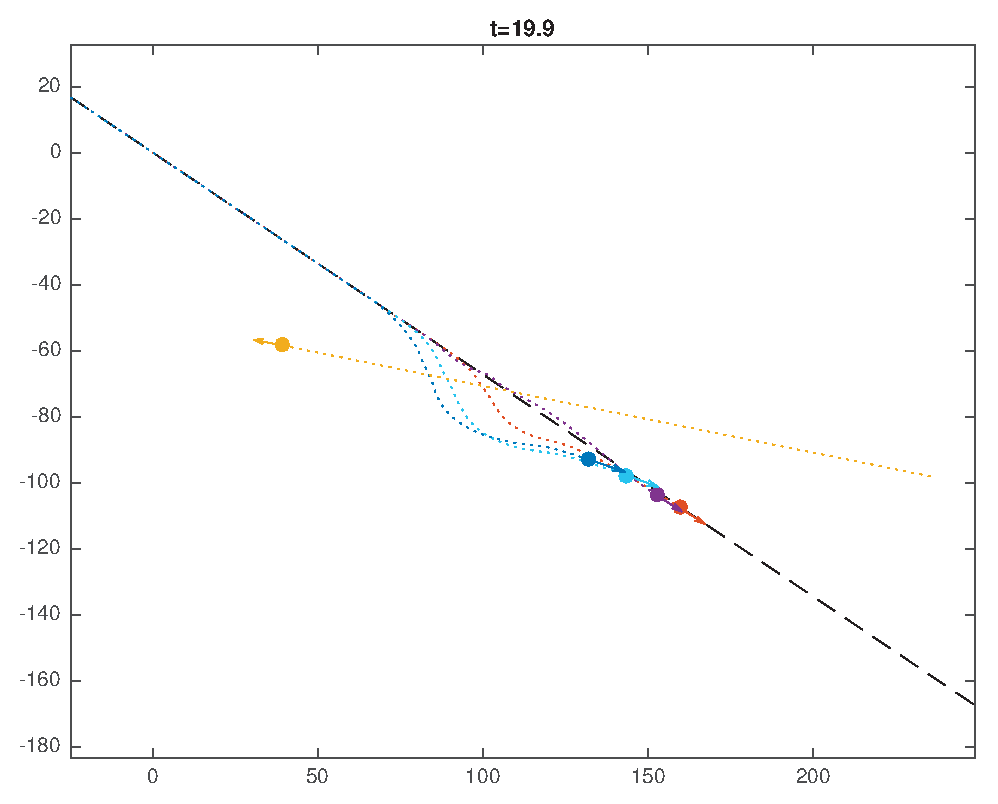
\includegraphics[width=\textwidth]{fig/in_200}
        \caption{After danger has passed, the platoon resumes normal operation.}
    \end{subfigure}   
    \caption{A simulation showing how a platoon of four vehicles react to an intruder. \label{fig:in}}
\end{figure}

\subsubsection{Changing highways}
In order to travel from origin to destination, a vehicle may need to change highways several times before exiting an air highway system. In this simulation, shown in Figure \ref{fig:ch}, two platoons are traveling on two different highways that intersect. When the platoons are near the highway intersection, two of the vehicles in the four-vehicle platoon change highways and join the other platoon.

The $t=8.2$ plot shows the two platoons of vehicles traveling on the two air highways. One platoon has three vehicles, and the other has four vehicles. At $t=12.3$, the yellow vehicle begins steering off its original highway in order to join the other platoon. In terms of the hybrid systems modes, the yellow vehicle transitions from the Leader mode to the Follower mode. At the same time, the green vehicle transitions from the Follower mode to the Leader mode, since the previous platoon leader, the yellow vehicle, has left the platoon. By $t=16.9$, the yellow vehicle successfully changes highways and is now a follower in its new platoon.

At $t=16.9$, the dark red vehicle is in the process of changing highways. In this case, it remains in the Follower mode, since it is a follower in both its old and new platoons. While the dark red vehicle changes highways, the orange vehicle moves forward to catch up to its new platoon leader, the green vehicle. By $t=23$, all the vehicles have finished performing their desired maneuvers, resulting in a two-vehicle platoon and a five-vehicle platoon traveling on their respective highways.

\begin{figure}
    \centering
    \begin{subfigure}[t]{0.45\textwidth} \label{subfig:ch_83}
        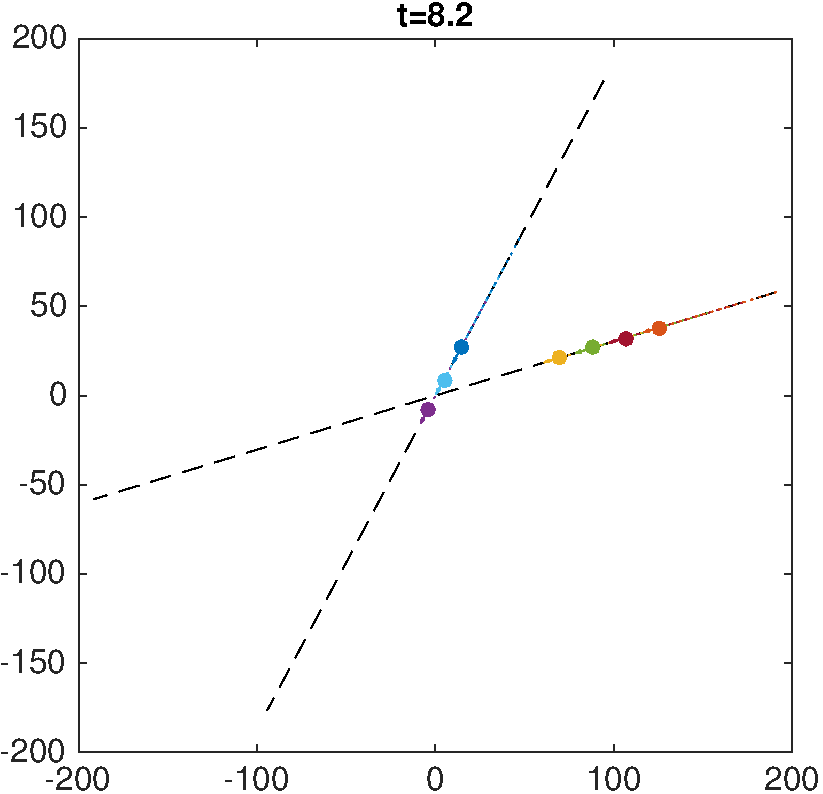
\includegraphics[width=\textwidth]{fig/ch_83}
        \caption{A three-vehicle platoon and a four-vehicle platoon are traveling on their respective air highways.}
    \end{subfigure}
    \begin{subfigure}[t]{0.45\textwidth} \label{subfig:ch_124}
        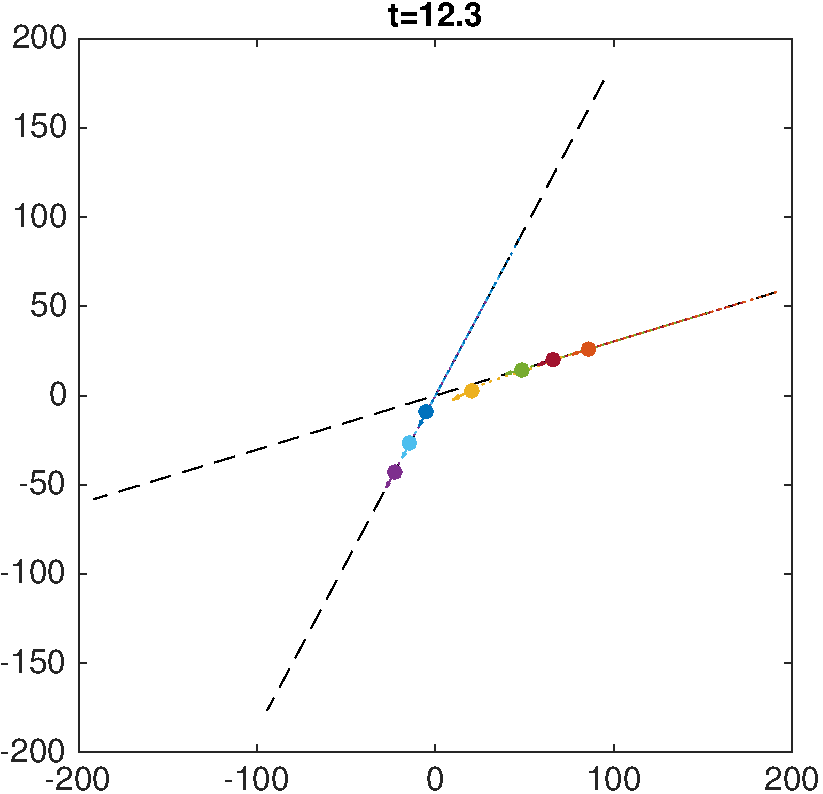
\includegraphics[width=\textwidth]{fig/ch_124}
        \caption{As the four-vehicle platoon nears the intersection, the yellow vehicle steers off its old highway to join the new platoon. The green vehicle becomes the old platoon's new leader.}
    \end{subfigure}

    \begin{subfigure}[t]{0.45\textwidth} \label{subfig:ch_170}
        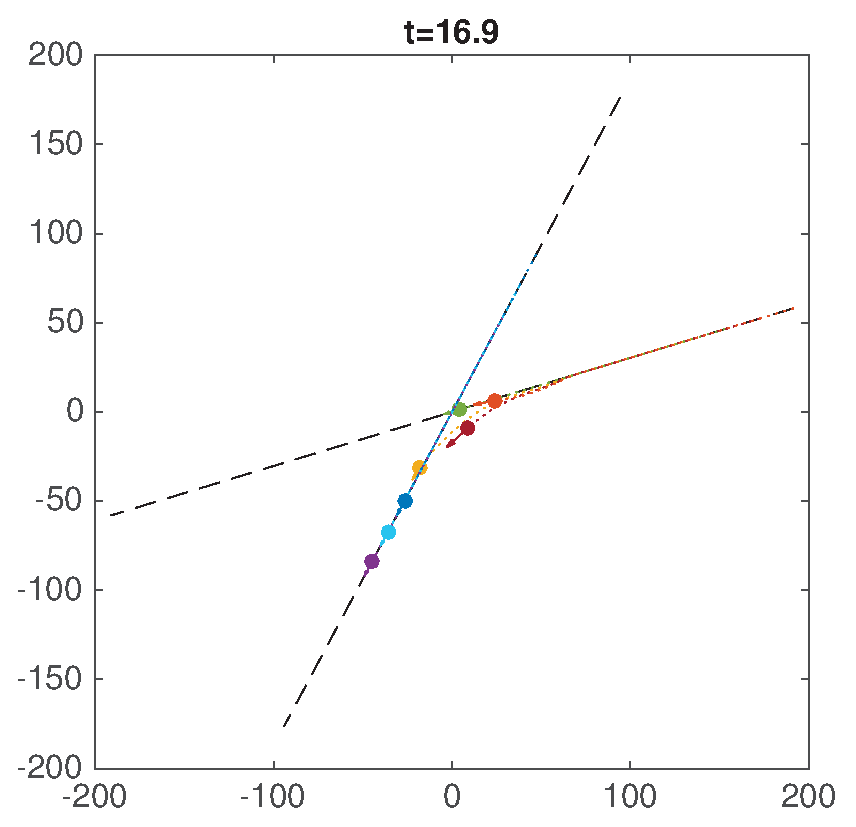
\includegraphics[width=\textwidth]{fig/ch_170}
        \caption{The dark red vehicle also changes highways to join a new platoon, while the orange vehicle catches up to the new platoon leader to maintain a proper formation.}
    \end{subfigure}
    \begin{subfigure}[t]{0.45\textwidth} \label{subfig:ch_231}
        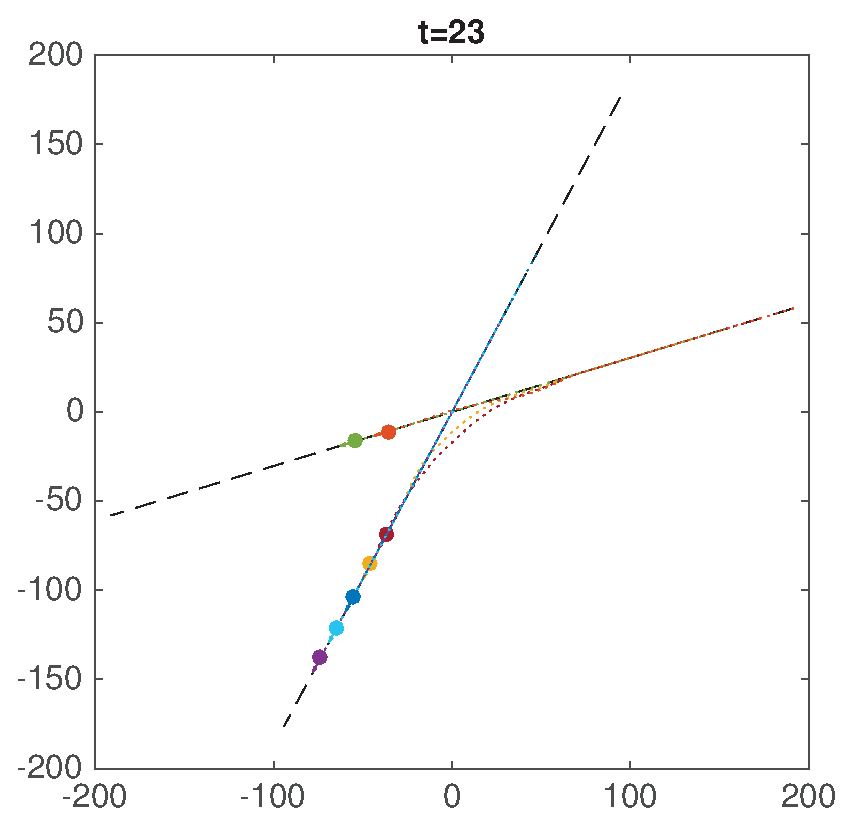
\includegraphics[width=\textwidth]{fig/ch_231}
        \caption{New platoons now travel on their respective air highways.}
    \end{subfigure}   
    \caption{A simulation showing two vehicles changing highways and joining a new platoon. \label{fig:ch}}
\end{figure}
